\section{Progetto}
\label{project}

Il progetto è composto da 5 sezioni:
\begin{itemize}
\item\emph{graph}
\item\emph{distance}
%\item\emph{movielens\_exp}
\item\emph{profile}
\item\emph{recommendation}
\end{itemize}

\subsection{graph}
Nella parte iniziale del progetto verranno eseguiti dei metodi presenti nella classi situate all'interno del package \emph{graph}, i cui scopi saranno quelli di:
\begin{itemize}
\item Salvare all'interno di un grafo i film presenti nel db di movielens\footnote{\emph{\url{http://www.grouplens.org/node/73}}};
\item A partire dal grafo creato in precedenza, si va a creare un nuovo grafo in cui ogni vertice rappresenta un film, mentre ogni arco rappresenta un possibile collegamento che intercorre tra due film attraverso un qualunque tipo di risorsa quale ad esempio un particolare attore facente parte del casting di entrambi i film presi in considerazione.
\end{itemize}

Al fine di soddisfare il primo obiettivo, all'interno della classe \textsc{Graph} sarà presente un metodo atto alla creazione del multigrafo sparso non direzionato attraverso l'esecuzione di query SPARQL utilizzando come endpoint il link di Dbpedia (\emph{\footnotesize{\url{http://dbpedia.org/sparql}}}).

Il risultato di questa computazione sarà un multigrafo avente come vertice risorse quali film,attori,case produttrici,registi,ecc; mentre come arco un predicato che mette in relazione le due risorse quale ad esempio director,writer,music composer e cosi via.

Per quanto riguarda il secondo obiettivo,all'interno della classe \textsc{FilmGraph} sarà presente un metodo il cui scopo sarà quello di convertire il multigrafo sparso non direzionato, in un nuovo multigrafo sparso direzionato i cui vertici saranno solo i film presenti nel db di movielens, mentre i cui archi saranno creati relazionando tra loro due archi definiti in precedenza aventi come soggetto della prima proprietà il film di partenza e come oggetto della seconda proprietà il film di destinazione.

\begin{figure}[H]
	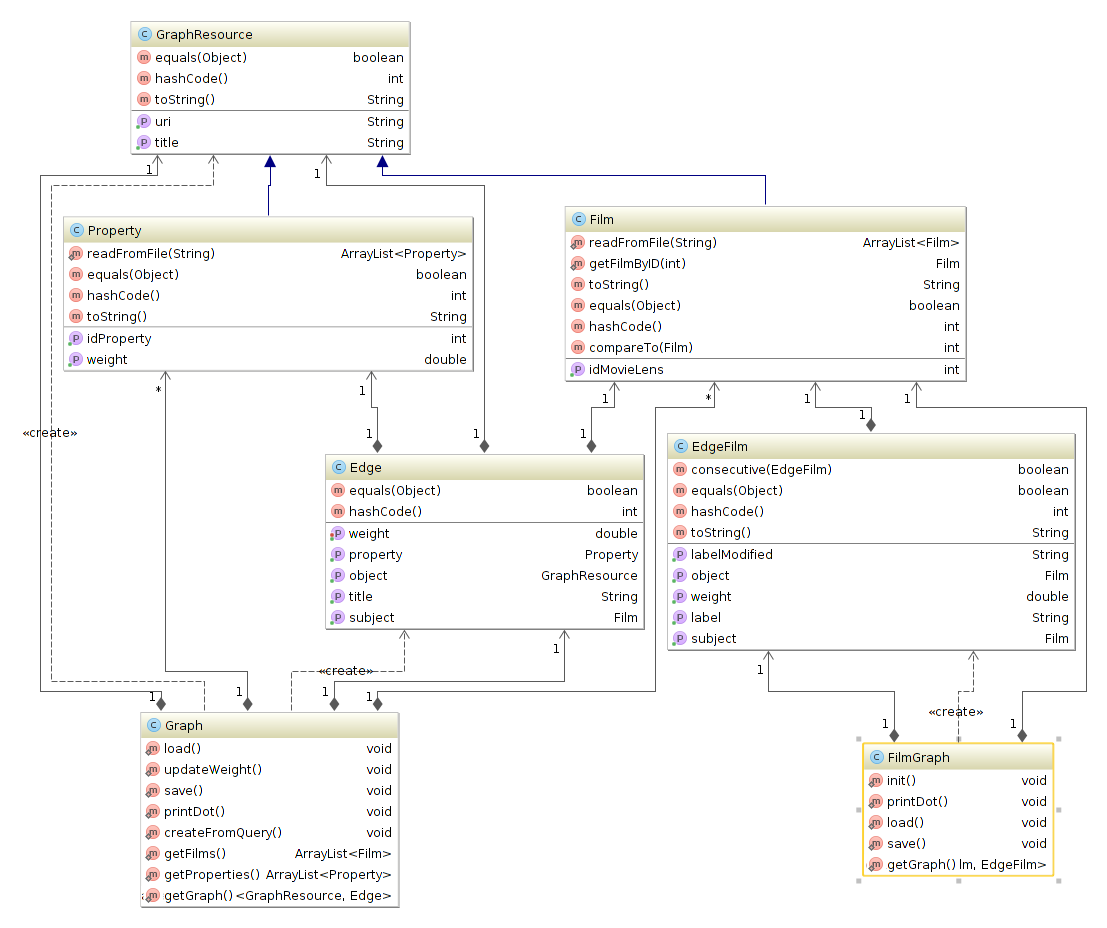
\includegraphics[width=\textwidth]{./images/Diagrams/graph.png}
	\caption{\emph{Class diagram: Package graph}}
\end{figure}

\subsection{distance}
Il compito principale di questo package è quello di creare sia tutte le distanze di Passant (verranno definite nel dettaglio nei paragrafi \ref{PassantD} e \ref{PassantC}), sia le distanze da noi implementate (\ref{PassantDW} e \ref{PassantCW}).
\begin{figure}[H]
	\advance\leftskip-3cm
	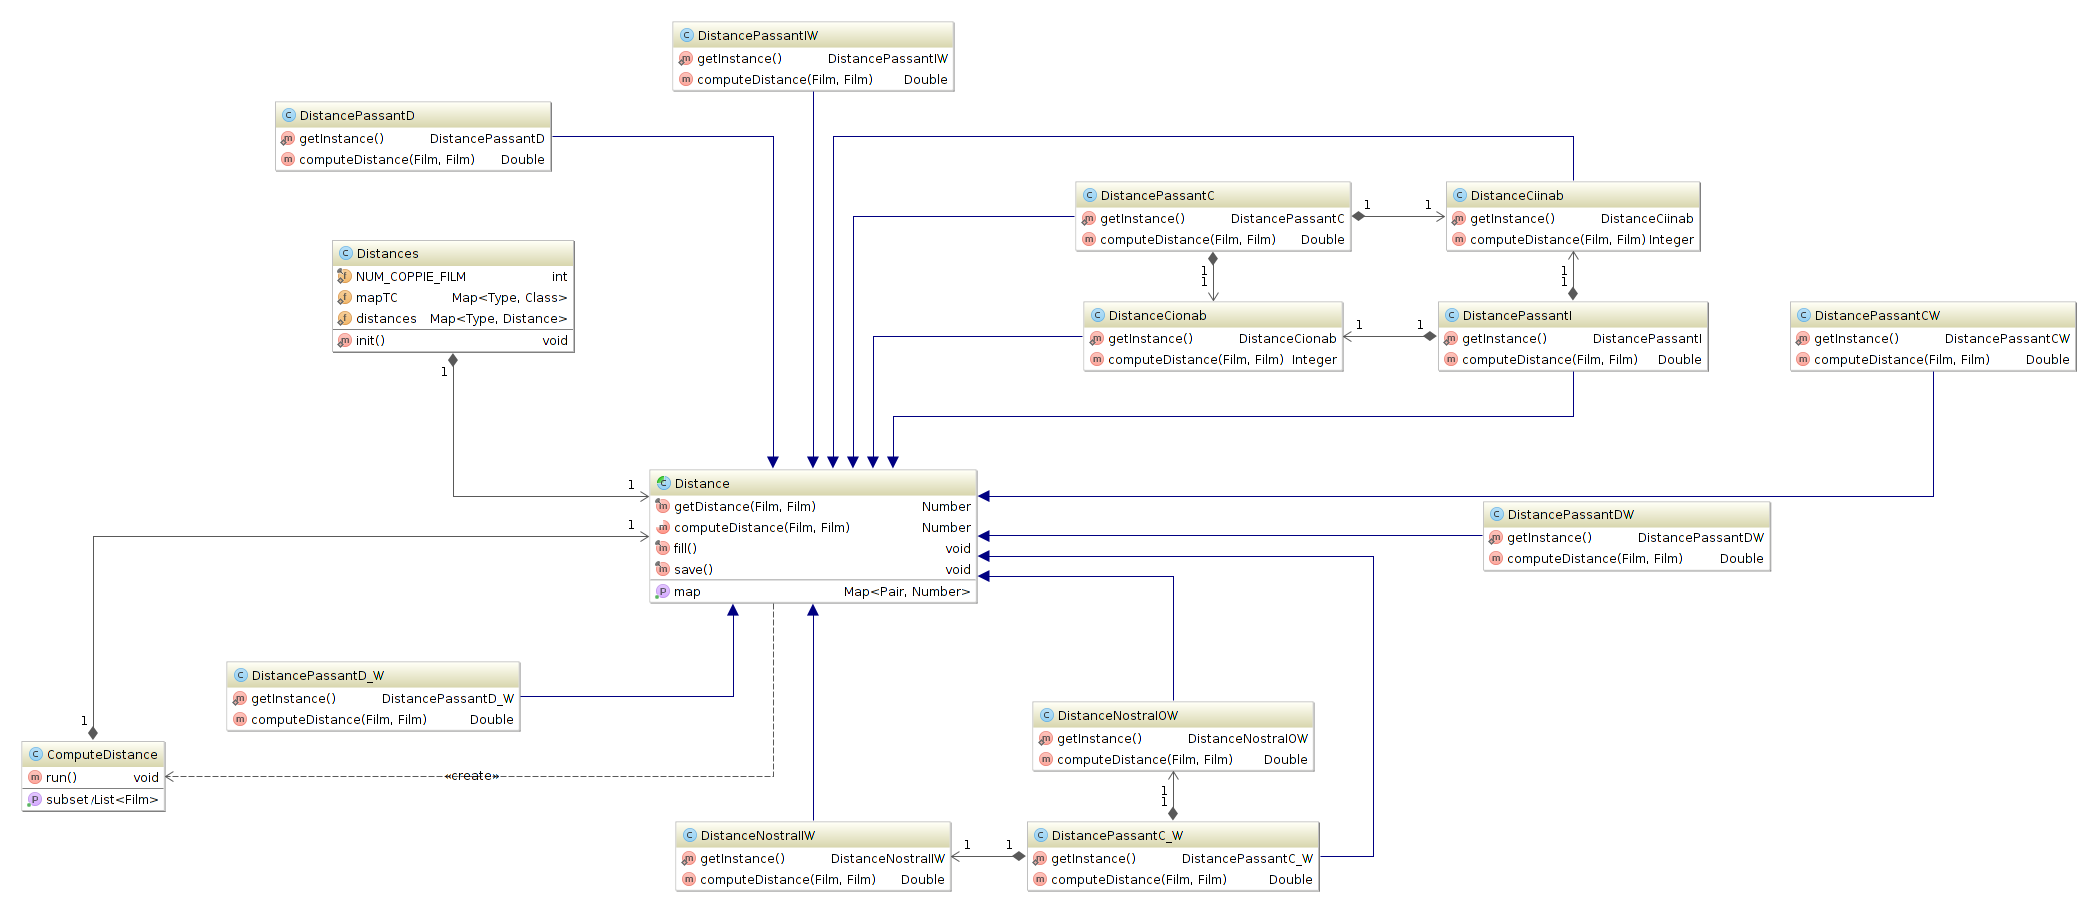
\includegraphics[width=1.45\textwidth]{./images/Diagrams/distance.png}
	\caption{\emph{Class diagram: Package distance}}
\end{figure}

\subsection{profile}
Tramite le classi presenti all'interno di questo package, sarà possibile implementare le due tipologie di profilo (pesato e non pesato)(verranno descritte in dettaglio nel paragrafo \ref{profili}).
\begin{figure}[H]
	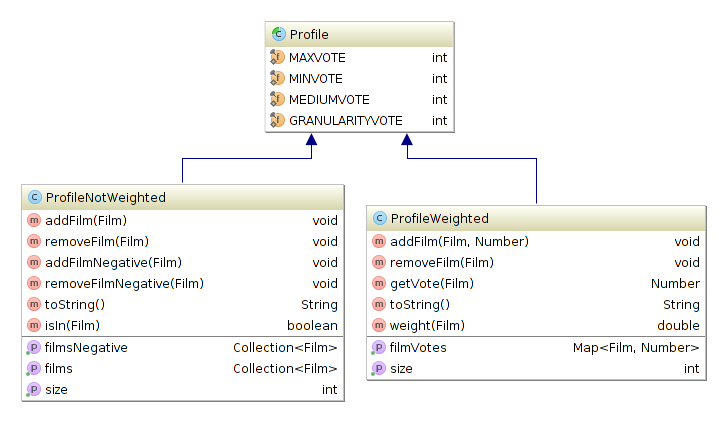
\includegraphics[width=\textwidth]{./images/Diagrams/profile.png}
	\caption{\emph{Class diagram: Package profile}}
\end{figure}

\subsection{recommendation}
Come dice il nome stesso, il compito di questo package consiste nella vera e propria fase di raccomandazione ad un utente partendo da una particolare configurazione. Per configurazione si intende definire innanzitutto ia tipologia di \emph{\textbf{distanza}} da utilizzare, poi si va definire quale tipo di profilo utente utilizzare (\emph{\textbf{pesato}} o \emph{\textbf{non pesato}}) e infine il numero \emph{\textbf{k}} di raccomandazioni da generare.

%\subsection{movielens\_exp}
%Il package \emph{movielens\_exp} ha il compito di eseguire la fase sperimentale del progetto; innanzitutto viene eseguita la fase di splitting delle votazioni date da ogni utente ai vari film visionati allo scopo di creare i set di training e di test. Successivamente si passa alla creazione dei profili(\emph{pesato} e \emph{non pesato}) partendo dalle votazioni presenti all'interno del training set di ogni utente; infine nella parte finale della sperimentazione vengono calcolate le diverse tipologie di metriche descritte in \ref{metriche}.

